%% bare_conf.tex
%% V1.4a
%% 2014/09/17
%% by Michael Shell
%% See:
%% http://www.michaelshell.org/
%% for current contact information.
%%
%% This is a skeleton file demonstrating the use of IEEEtran.cls
%% (requires IEEEtran.cls version 1.8a or later) with an IEEE
%% conference paper.
%%
%% Support sites:
%% http://www.michaelshell.org/tex/ieeetran/
%% http://www.ctan.org/tex-archive/macros/latex/contrib/IEEEtran/
%% and
%% http://www.ieee.org/

%%*************************************************************************
%% Legal Notice:
%% This code is offered as-is without any warranty either expressed or
%% implied; without even the implied warranty of MERCHANTABILITY or
%% FITNESS FOR A PARTICULAR PURPOSE! 
%% User assumes all risk.
%% In no event shall IEEE or any contributor to this code be liable for
%% any damages or losses, including, but not limited to, incidental,
%% consequential, or any other damages, resulting from the use or misuse
%% of any information contained here.
%%
%% All comments are the opinions of their respective authors and are not
%% necessarily endorsed by the IEEE.
%%
%% This work is distributed under the LaTeX Project Public License (LPPL)
%% ( http://www.latex-project.org/ ) version 1.3, and may be freely used,
%% distributed and modified. A copy of the LPPL, version 1.3, is included
%% in the base LaTeX documentation of all distributions of LaTeX released
%% 2003/12/01 or later.
%% Retain all contribution notices and credits.
%% ** Modified files should be clearly indicated as such, including  **
%% ** renaming them and changing author support contact information. **
%%
%% File list of work: IEEEtran.cls, IEEEtran_HOWTO.pdf, bare_adv.tex,
%%                    bare_conf.tex, bare_jrnl.tex, bare_conf_compsoc.tex,
%%                    bare_jrnl_compsoc.tex, bare_jrnl_transmag.tex
%%*************************************************************************


% *** Authors should verify (and, if needed, correct) their LaTeX system  ***
% *** with the testflow diagnostic prior to trusting their LaTeX platform ***
% *** with production work. IEEE's font choices and paper sizes can       ***
% *** trigger bugs that do not appear when using other class files.       ***                          ***
% The testflow support page is at:
% http://www.michaelshell.org/tex/testflow/



\documentclass[11pt, a4paper]{IEEEtran}
% Some Computer Society conferences also require the compsoc mode option,
% but others use the standard conference format.
%
% If IEEEtran.cls has not been installed into the LaTeX system files,
% manually specify the path to it like:
% \documentclass[conference]{../sty/IEEEtran}



% Some very useful LaTeX packages include:
% (uncomment the ones you want to load)


% *** MISC UTILITY PACKAGES ***
%
%\usepackage{ifpdf}
% Heiko Oberdiek's ifpdf.sty is very useful if you need conditional
% compilation based on whether the output is pdf or dvi.
% usage:
% \ifpdf
%   % pdf code
% \else
%   % dvi code
% \fi
% The latest version of ifpdf.sty can be obtained from:
% http://www.ctan.org/tex-archive/macros/latex/contrib/oberdiek/
% Also, note that IEEEtran.cls V1.7 and later provides a builtin
% \ifCLASSINFOpdf conditional that works the same way.
% When switching from latex to pdflatex and vice-versa, the compiler may
% have to be run twice to clear warning/error messages.






% *** CITATION PACKAGES ***
%
%\usepackage{cite}
% cite.sty was written by Donald Arseneau
% V1.6 and later of IEEEtran pre-defines the format of the cite.sty package
% \cite{} output to follow that of IEEE. Loading the cite package will
% result in citation numbers being automatically sorted and properly
% "compressed/ranged". e.g., [1], [9], [2], [7], [5], [6] without using
% cite.sty will become [1], [2], [5]--[7], [9] using cite.sty. cite.sty's
% \cite will automatically add leading space, if needed. Use cite.sty's
% noadjust option (cite.sty V3.8 and later) if you want to turn this off
% such as if a citation ever needs to be enclosed in parenthesis.
% cite.sty is already installed on most LaTeX systems. Be sure and use
% version 5.0 (2009-03-20) and later if using hyperref.sty.
% The latest version can be obtained at:
% http://www.ctan.org/tex-archive/macros/latex/contrib/cite/
% The documentation is contained in the cite.sty file itself.






% *** GRAPHICS RELATED PACKAGES ***
%
\ifCLASSINFOpdf
  % \usepackage[pdftex]{graphicx}
  % declare the path(s) where your graphic files are
  % \graphicspath{{../pdf/}{../jpeg/}}
  % and their extensions so you won't have to specify these with
  % every instance of \includegraphics
  % \DeclareGraphicsExtensions{.pdf,.jpeg,.png}
\else
  % or other class option (dvipsone, dvipdf, if not using dvips). graphicx
  % will default to the driver specified in the system graphics.cfg if no
  % driver is specified.
  % \usepackage[dvips]{graphicx}
  % declare the path(s) where your graphic files are
  % \graphicspath{{../eps/}}
  % and their extensions so you won't have to specify these with
  % every instance of \includegraphics
  % \DeclareGraphicsExtensions{.eps}
\fi
% graphicx was written by David Carlisle and Sebastian Rahtz. It is
% required if you want graphics, photos, etc. graphicx.sty is already
% installed on most LaTeX systems. The latest version and documentation
% can be obtained at: 
% http://www.ctan.org/tex-archive/macros/latex/required/graphics/
% Another good source of documentation is "Using Imported Graphics in
% LaTeX2e" by Keith Reckdahl which can be found at:
% http://www.ctan.org/tex-archive/info/epslatex/
%
% latex, and pdflatex in dvi mode, support graphics in encapsulated
% postscript (.eps) format. pdflatex in pdf mode supports graphics
% in .pdf, .jpeg, .png and .mps (metapost) formats. Users should ensure
% that all non-photo figures use a vector format (.eps, .pdf, .mps) and
% not a bitmapped formats (.jpeg, .png). IEEE frowns on bitmapped formats
% which can result in "jaggedy"/blurry rendering of lines and letters as
% well as large increases in file sizes.
%
% You can find documentation about the pdfTeX application at:
% http://www.tug.org/applications/pdftex





% *** MATH PACKAGES ***
%
%\usepackage[cmex10]{amsmath}
% A popular package from the American Mathematical Society that provides
% many useful and powerful commands for dealing with mathematics. If using
% it, be sure to load this package with the cmex10 option to ensure that
% only type 1 fonts will utilized at all point sizes. Without this option,
% it is possible that some math symbols, particularly those within
% footnotes, will be rendered in bitmap form which will result in a
% document that can not be IEEE Xplore compliant!
%
% Also, note that the amsmath package sets \interdisplaylinepenalty to 10000
% thus preventing page breaks from occurring within multiline equations. Use:
%\interdisplaylinepenalty=2500
% after loading amsmath to restore such page breaks as IEEEtran.cls normally
% does. amsmath.sty is already installed on most LaTeX systems. The latest
% version and documentation can be obtained at:
% http://www.ctan.org/tex-archive/macros/latex/required/amslatex/math/





% *** SPECIALIZED LIST PACKAGES ***
%
%\usepackage{algorithmic}
% algorithmic.sty was written by Peter Williams and Rogerio Brito.
% This package provides an algorithmic environment fo describing algorithms.
% You can use the algorithmic environment in-text or within a figure
% environment to provide for a floating algorithm. Do NOT use the algorithm
% floating environment provided by algorithm.sty (by the same authors) or
% algorithm2e.sty (by Christophe Fiorio) as IEEE does not use dedicated
% algorithm float types and packages that provide these will not provide
% correct IEEE style captions. The latest version and documentation of
% algorithmic.sty can be obtained at:
% http://www.ctan.org/tex-archive/macros/latex/contrib/algorithms/
% There is also a support site at:
% http://algorithms.berlios.de/index.html
% Also of interest may be the (relatively newer and more customizable)
% algorithmicx.sty package by Szasz Janos:
% http://www.ctan.org/tex-archive/macros/latex/contrib/algorithmicx/




% *** ALIGNMENT PACKAGES ***
%
%\usepackage{array}
% Frank Mittelbach's and David Carlisle's array.sty patches and improves
% the standard LaTeX2e array and tabular environments to provide better
% appearance and additional user controls. As the default LaTeX2e table
% generation code is lacking to the point of almost being broken with
% respect to the quality of the end results, all users are strongly
% advised to use an enhanced (at the very least that provided by array.sty)
% set of table tools. array.sty is already installed on most systems. The
% latest version and documentation can be obtained at:
% http://www.ctan.org/tex-archive/macros/latex/required/tools/


% IEEEtran contains the IEEEeqnarray family of commands that can be used to
% generate multiline equations as well as matrices, tables, etc., of high
% quality.




% *** SUBFIGURE PACKAGES ***
%\ifCLASSOPTIONcompsoc
%  \usepackage[caption=false,font=normalsize,labelfont=sf,textfont=sf]{subfig}
%\else
%  \usepackage[caption=false,font=footnotesize]{subfig}
%\fi
% subfig.sty, written by Steven Douglas Cochran, is the modern replacement
% for subfigure.sty, the latter of which is no longer maintained and is
% incompatible with some LaTeX packages including fixltx2e. However,
% subfig.sty requires and automatically loads Axel Sommerfeldt's caption.sty
% which will override IEEEtran.cls' handling of captions and this will result
% in non-IEEE style figure/table captions. To prevent this problem, be sure
% and invoke subfig.sty's "caption=false" package option (available since
% subfig.sty version 1.3, 2005/06/28) as this is will preserve IEEEtran.cls
% handling of captions.
% Note that the Computer Society format requires a larger sans serif font
% than the serif footnote size font used in traditional IEEE formatting
% and thus the need to invoke different subfig.sty package options depending
% on whether compsoc mode has been enabled.
%
% The latest version and documentation of subfig.sty can be obtained at:
% http://www.ctan.org/tex-archive/macros/latex/contrib/subfig/




% *** FLOAT PACKAGES ***
%
%\usepackage{fixltx2e}
% fixltx2e, the successor to the earlier fix2col.sty, was written by
% Frank Mittelbach and David Carlisle. This package corrects a few problems
% in the LaTeX2e kernel, the most notable of which is that in current
% LaTeX2e releases, the ordering of single and double column floats is not
% guaranteed to be preserved. Thus, an unpatched LaTeX2e can allow a
% single column figure to be placed prior to an earlier double column
% figure. The latest version and documentation can be found at:
% http://www.ctan.org/tex-archive/macros/latex/base/


%\usepackage{stfloats}
% stfloats.sty was written by Sigitas Tolusis. This package gives LaTeX2e
% the ability to do double column floats at the bottom of the page as well
% as the top. (e.g., "\begin{figure*}[!b]" is not normally possible in
% LaTeX2e). It also provides a command:
%\fnbelowfloat
% to enable the placement of footnotes below bottom floats (the standard
% LaTeX2e kernel puts them above bottom floats). This is an invasive package
% which rewrites many portions of the LaTeX2e float routines. It may not work
% with other packages that modify the LaTeX2e float routines. The latest
% version and documentation can be obtained at:
% http://www.ctan.org/tex-archive/macros/latex/contrib/sttools/
% Do not use the stfloats baselinefloat ability as IEEE does not allow
% \baselineskip to stretch. Authors submitting work to the IEEE should note
% that IEEE rarely uses double column equations and that authors should try
% to avoid such use. Do not be tempted to use the cuted.sty or midfloat.sty
% packages (also by Sigitas Tolusis) as IEEE does not format its papers in
% such ways.
% Do not attempt to use stfloats with fixltx2e as they are incompatible.
% Instead, use Morten Hogholm'a dblfloatfix which combines the features
% of both fixltx2e and stfloats:
%
% \usepackage{dblfloatfix}
% The latest version can be found at:
% http://www.ctan.org/tex-archive/macros/latex/contrib/dblfloatfix/


%% Language and font encodings
\usepackage[ngerman, english]{babel}
\usepackage[utf8x]{inputenc}
\usepackage[T1]{fontenc}

%% Sets page size and margins
\usepackage[a4paper,top=3cm,bottom=2cm,left=3cm,right=3cm,marginparwidth=1.75cm]{geometry}

%% Useful packages
\usepackage{amsmath}
\usepackage{graphicx}
\usepackage[colorinlistoftodos]{todonotes}
\usepackage{xpatch}
\usepackage[hyphens]{url}
\usepackage[colorlinks=true, allcolors=blue]{hyperref}
\usepackage{tabularx}
\usepackage{float}
\usepackage{enumitem}
% *** PDF, URL AND HYPERLINK PACKAGES ***
%
%\usepackage{url}
% url.sty was written by Donald Arseneau. It provides better support for
% handling and breaking URLs. url.sty is already installed on most LaTeX
% systems. The latest version and documentation can be obtained at:
% http://www.ctan.org/tex-archive/macros/latex/contrib/url/
% Basically, \url{my_url_here}.




% *** Do not adjust lengths that control margins, column widths, etc. ***
% *** Do not use packages that alter fonts (such as pslatex).         ***
% There should be no need to do such things with IEEEtran.cls V1.6 and later.
% (Unless specifically asked to do so by the journal or conference you plan
% to submit to, of course. )


% correct bad hyphenation here
\hyphenation{op-tical net-works semi-conduc-tor}



\begin{document}


%
% paper title
% Titles are generally capitalized except for words such as a, an, and, as,
% at, but, by, for, in, nor, of, on, or, the, to and up, which are usually
% not capitalized unless they are the first or last word of the title.
% Linebreaks \\ can be used within to get better formatting as desired.
% Do not put math or special symbols in the title.
\title{Introduction to Holographic Devices}


% author names and affiliations
% use a multiple column layout for up to three different
% affiliations
\author{
\IEEEauthorblockN{
Peter Enenkel\IEEEauthorrefmark{1},
André Höfler\IEEEauthorrefmark{2} and 
Mario Miosga\IEEEauthorrefmark{3}
}

\IEEEauthorblockA{Fachbereich Informatik,
Hochschule Darmstadt\\
Haardtring 100, 64295 Darmstadt\\
Email:
\IEEEauthorrefmark{1}\href{mailto:peter.enenkel@stud.h-da.de}{peter.enenkel@stud.h-da.de}
\IEEEauthorrefmark{2}\href{mailto:andre.m.hoefler@stud.h-da.de}{andre.m.hoefler@stud.h-da.de}
\IEEEauthorrefmark{3}\href{mailto:mario.miosga@stud.h-da.de}{mario.miosga@stud.h-da.de}}
}

%\author{
%
%	\IEEEauthorblockN{Peter Enenkel}
%	\IEEEauthorblockA{Hochschule Darmstadt\\
%		Haardtring 100, 64295 Darmstadt\\
%		Email: \href{mailto:peter.enenkel@stud.h-da.de}{peter.enenkel@stud.h-da.de}
%        }\\
%        
%    \IEEEauthorblockN{André Höfler}
%	\IEEEauthorblockA{Hochschule Darmstadt\\
%		Haardtring 100, 64295 Darmstadt\\
%		Email: \href{mailto:andre.m.hoefler@stud.h-da.de}{andre.m.hoefler@stud.h-da.de}
%        }\and
%	\IEEEauthorblockN{Mario Miosga}
%	\IEEEauthorblockA{Hochschule Darmstadt\\
%		Haardtring 100, 64295 Darmstadt\\
%		Email: \href{mailto:mario.miosga@stud.h-da.de}{mario.miosga@stud.h-da.de}
%        }
%}

% use for special paper notices
%\IEEEspecialpapernotice{(Invited Paper)}

% force page number to title page 
\patchcmd{\titlepage}
  {\thispagestyle{empty}}
  {\thispagestyle{plain}}
  {}
  {}

% make the title area
\maketitle
\thispagestyle{plain}
\pagestyle{plain}

% As a general rule, do not put math, special symbols or citations
% in the abstract
%\begin{abstract}
%The abstract goes here.
%\end{abstract}

% no keywords




% For peer review papers, you can put extra information on the cover
% page as needed:
% \ifCLASSOPTIONpeerreview
% \begin{center} \bfseries EDICS Category: 3-BBND \end{center}
% \fi
%
% For peerreview papers, this IEEEtran command inserts a page break and
% creates the second title. It will be ignored for other modes.
\IEEEpeerreviewmaketitle

\begin{abstract}
As holographic devices gain more and more exposure, people of all areas of expertise are looking into utilizing them. To help them gain traction with this emerging technology this article provides an easy to follow introduction. To that purpose we introduce and differentiate the various relevant technical terms, present the inherent technological difficulties as well as discuss some realistically achievable goals. Further a concrete starting point is provided by presenting a non exhaustive and biased selection of devices, which in our opinion represent the commercially available state-of-the-art.
\end{abstract}


\section{Introduction}
When surveying the market for head-mounted holographic devices there are several aspects to be considered: Is the projected scene entirely virtual or mixed with reality? Does the virtual content consist of two or three dimensional objects? Are those objects anchored in the reality or not? Is the device fully mobile or tethered to a computer? How does the user interact with the holographic content? 

To help with understanding and answering these questions we begin with establishing the most relevant concepts and terms in section \ref{sec:concepts}. In the subsequent section \ref{sec:limitations} we inform about where the current technological limitations lie and what can realistically be expected. We then present selection of state-of-the-art devices in section \ref{sec:stateoftheart} and close with some concluding remarks in section \ref{sec:end}.



\section{Terminology and Concepts}\label{sec:concepts}
The precise terminology for holographic devices is currently in flux. Mostly due to the fact that more and more devices are released, each with slightly different capabilities. Conceptually the spectrum spans from plain old \emph{reality} at one end to an entirely \emph{virtual reality} (VR) at the other end. Any combination of reality with virtual elements is known as either \emph{augmented reality} (AR) or \emph{mixed reality} (MR) interchangeably. The devices for all three technologies look quite similar. Most of them are build like large front-heavy glasses. See section \ref{sec:stateoftheart} for some images.

\subsection{Virtual Reality}
Virtual reality headsets completely shut the wearer off from the environment. This allows for a totally immersive experience and the delivery of 360 degree views of artificial virtual worlds. Sensory input from the outside wold is usually minimal and always filtered through the device. VR headsets are heavily represented in the gaming sector, where they are mostly soled as accessors to gaming consoles and computers. 

\subsection{Augmented vs. Mixed  Reality}
Augmented and mixed reality devices add 2D and/or 3D holographic content to the normal view. As such they kind of resemble heavy wraparound sunglasses. The user is still able to see his surroundings almost as well as without the device. This still holds true if the device is turned off.

While it is usually valid to use augmented and mixed reality interchangeably, Microsoft recently  sharped their understanding of the nomenclature. They now differentiate between augmented and mixed reality by referring to reality enriched with 2D holographic content as augmented reality and using the term mixed reality exclusively for systems with 3D holographic content which is also anchorable in reality. Other manufacturers have yet to adopt this nomenclature.

\subsection{Anchoring and Spatial Mapping}
Anchoring, as used above, refers to the technique of attaching holographic content to a precise location in reality. This is used to either attach holographic labels to real-world objects or to overlay them entirely with a hologram. To make this possible continuous mapping and tracking of the environment is required, which is commonly referred to as \emph{spatial mapping}. Depending on the required precision and update rate this is a computationally challenging task on which we will elaborate in section \ref{sec:limitations}.

\subsection{Tethered vs. Untethered}
%Augmented Reality (AR) and Virtual Reality (VR) are a thriving topic these days. Currently there are a lot of different devices on the Market and, at a closer look, they are more differences than it seems. 
An other distinguishing characteristic is whether the device is tethered or not. Tethered devices are cable-bound and rely on an external computation unit (i.e. computer) to provide the necessary processing and rendering power. Untethered devices on the other hand are mobile devices in the truest sense with all the inherent advantages and disadvantages. The main advantage of an untethered device is the freedom it provides. You can walk around and use it anywhere. The downsides are the limitations in computing power (which is about the same as a smartphone) and the limited battery life. In fact many of the untethered VR devices are actually simply a mounting platform for a smartphone. Examples for unthered devices are \textit{Microsoft's HoloLens} (AR), \textit{Samsung's GearVR} (VR) and \textit{Google's Daydream} (VR). We will elaborate on our impressions of working with the \textit{HoloLens} in section \ref{sec:stateoftheart}.

Tethered devices do not have those limitations. They can be combined with an arbitrarily powerful desktop computer with maybe multiple high-end graphics cards and CPUs and an effectively infinite power supply. The obvious downside is that the user is on a leash of (sometimes severely) limited length. Samples for cable-bound devices are the \textit{Meta 2} (AR), the \textit{HTC Vive} (VR) and the \textit{Oculus Rift} (VR). All of which will be presented in more detail in section \ref{sec:stateoftheart}.

\section{Limitations}\label{sec:limitations}
This chapter addresses the gap between expected and achievable performance and features.
\subsection{Expectations}
Influenced by literature, film and TV a lot of people tend to have a quite definitive notion of what virtual or augmented reality is or at least could be. In itself that is a good thing as it serves as a common vision of what is to be attained. Problematic from our point of view is that it creates false expectations of what is currently doable with state-of-the-art hardware. The situation is exacerbated by the many promotional videos for new and upcoming holographic devices that have more in common with Hollywood productions than with the devices actual capabilities. The presented features and functionalities are often so significantly exaggerated, especially with regard to resolution, smoothness of interaction and field-of-view, that they are practically useless for evaluating and comparing. As a consequence, Whenever a wide-angle shot of a room full of moving high-definition holograms is shown, the discerning viewer should become instantly skeptical, as this is simply not feasible at this point in time.

\subsection{Difficulties}
One of the most commonly underestimated difficulties with augmented or mixed reality is attaching holographic content to reality, especially if precise positioning is required. Which in general requires recognition and tracking of surfaces and objects, in real-time and with sufficient accuracy. 
This is a non trivial problem, even more so if both camera/viewer and observed object may move about freely. Anything based on image recognition requires large amounts of computing power. 

For mobile devices the traditional limitations also apply: With limited size and weight, endurance and performance are limited as well. Fitting sensors, holographic display, sufficient processing power as well as a large enough power supply into a wearable mobile device is always a challenging task.

\subsection{Realistic Expectations}
Using specialized range imaging hardware (e.g. time of flight cameras) in addition to pure image processing helps alleviate some of the difficulties mentioned above, but the problem remains fairly complex and more importantly computationally expensive. Nevertheless some astonishing results can be achieved if only the goal is defined sufficiently narrow. 

For example it is certainly possible to support real-time object detection, provided the number of objects is low enough and provided the objects are known beforehand, e.g. by providing CAD models of them. In such cases an artificial neural network could be trained in advance on a more powerful system and real-time tracking would then be possible even on limited hardware. But while this will work for a small number of distinct objects it won't for for hundreds or even dozens, as the network would have to be trained for each of them which would result in a huge amount of training data which in turn would have to be stored on the device. But if the chosen use-case only requires the detection of one precisely known object then it is solvable.


\section{State of the Art}\label{sec:stateoftheart}
In this section we will present a small selection of current, commercially available, devices. Representing mixed reality devices are the \textit{Microsoft HoloLens} \ref{subsec:holoLens} as an example of a fully mobile device and the \textit{Meta 2} \ref{subsec:meta2} as an example of a tethered device.  
Further we have included the \textit{Oculus Rift} and the \textit{HTC Vive} \ref{subsec:riftvive} which are both well established tethered virtual reality devices. All of those have in common that they are available right now and that they are placed at the upper end of the performance spectrum. We mostly choose those devices we have had some direct experience with. At the very least they have established enough of a track record that believable information is available. The \textit{Meta 2} was chosen because, even while on paper it seems quite similar to the \textit{HoloLens}, the interaction and usage concept appears to be totally different.


\subsection{Microsoft HoloLens}\label{subsec:holoLens}
Microsoft's HoloLens (Figure \ref{fig:holoLens}) is an untethered, standalone device. This makes it possible to use the headset anywhere. The HoloLens is capable of 3-5 hours continuous use depending on computational load before it has to be charged again. The most severe downside is the limitation in computing power. The interaction concept of the HoloLens is closely based on the point and click interface of common operating systems. The cursor is controlled by head movement instead of mouse or touchpad and a tap gesture replaces mouse clicks. A so called bloom gesture is comparable to the Windows-button or start menu. The only other supported gestures are two finger gestures for zoom an rotation. All in all the user interface is surprisingly lean if one considers how many separate gestures the average touch device supports. Microsoft recommends that developers should place holograms at least 80 centimeters from the device for a better user experience. In effect that creates an arm-length exclusion zone in which only hand gestures are supported.

The key feature of the HoloLens however is the build in environment awareness. While moving through a room the HoloLens builds and continuously updates a spatial map of the surroundings. Thus holograms can interact with the room in a limited fashion, e.g. balls rolling of tables and things like that. Those scans or mappings can also be saved and reused even for multiple rooms.
It should however be mentioned that the active scanning range is limited to about 2.5 meters.
\begin{table}[ht]
\caption{HoloLens Specifications}
\centering
\begin{tabularx}{\columnwidth}{p{0.25\columnwidth}X}
Resolution & 1268x720 per eye resolution (60 frames per second )\\
\hline
Field Of View & About 30°\\
\hline
Audio & Built-in speakers (Spatial sound)\\
\hline
Connections & Micro USB 2.0 for charging and data\\
\hline
	Sensors &
      \begin{tabular}[t]{@{\textbullet~}p{\linewidth}@{}}
     	1 IMU\\
      	4 environment understanding cameras\\
      	1 depth camera\\
      	1 2MP photo / HD video camera\\
      	Mixed reality capture\\
     	4 microphones\\
      	1 ambient light sensor
      \end{tabular}\\
\hline
	Power &
     \begin{tabular}[t]{@{\textbullet~}p{\linewidth}@{}}
      	 Battery Life\\
      	 2-3 hours of active use\\
      	 Up to 2 weeks of standby time\\
      	 Fully functional when charging\\
      	 Passively cooled (no fans)
     \end{tabular} \\
\hline
Processors  & 
	\begin{tabular}[t]{@{\textbullet~}p{\linewidth}@{}}
    	Intel 32 bit architecture with TPM 2.0 support\\
    	Custom-built Microsoft Holographic Processing Unit (HPU 1.0)
  	\end{tabular} \\
\hline
Memory &
	\begin{tabular}[t]{@{\textbullet~}p{\linewidth}@{}}
    	64GB Flash\\
    	2GB RAM
  	\end{tabular} \\
\end{tabularx}
\end{table}


\begin{figure}[ht]
\caption{HoloLens}
\label{fig:holoLens}
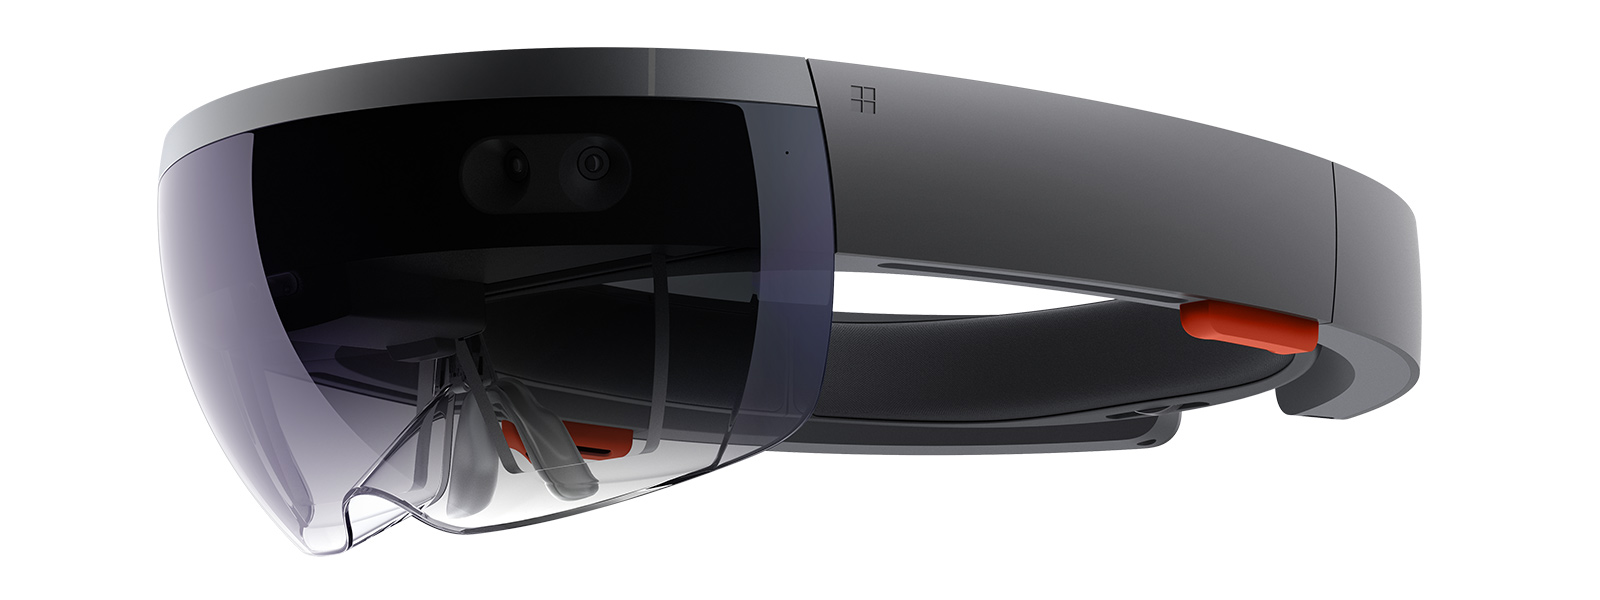
\includegraphics[width=\columnwidth]{images/hololens}
\end{figure}

%\newpage


\subsection{Meta 2}\label{subsec:meta2}
The Meta 2 (Figure \ref{fig:meta2}) is a tethered headset. This potentially provides a huge amount of computing power because any high-end desktop computer could be used. The downside is that one is tied rather closely (about 3 meters) to the computer. The interaction concept of the Meta 2 is radically different from that of the HoloLens instead of pointing and clicking the user can directly interact with the holograms by touching and grasping them. Obviously this limits the distance of interactive holograms to about arm-length. Which is basically an inversion of the recommendations for the HoloLens.

As previously stated environment awareness is one of the most important aspects of augmented reality. Unfortunately we were not able to find any reliable information on how the Meta 2 approaches this. In some of the promotional videos it seems like the Meta 2 has some kind of knowledge for objects right in front of the device. With regard to this the HoloLens seems much more capable (and better documented) as it can remember multiple rooms and knows in which one you currently are. But perhaps due to the fact that the Meta 2 is always tethered to a fixed point, such a feature is simply not necessary.

\begin{table}[ht]
\caption{Meta 2 Specifications}
\centering
  \begin{tabularx}{\columnwidth}{p{0.25\columnwidth}X}
    Resolution & 2550x1440 resolution (60 Hz refresh rate)\\
    \hline
    Field Of View & 90°\\
    \hline
    Audio & Four speaker near-ear audio system\\
    \hline
    Connections & HDMI for video, data and power\\
    \hline
    Sensors & 720p front-facing camera\\
    &Sensor array for hand interactions and positional tracking\\
    \hline
    Recommended PC Requirements & 
      \begin{tabular}[t]{@{\textbullet~}p{\linewidth}@{}}
      	Graphics: NVIDIA GTX 960 / AMD R9 280\\
      	CPU: Intel Core i7 (desktop CPU)\\
      	Memory: 8GB RAM\\
      	Game Engine: 64-bit Unity 5.3x\\
      	Storage: 10GB\\
      	Video: HDMI 1.4b\\
      	Sound Card: Intel HD-compatible sound card\\
      	USB Ports: USB 3.0\\
      	OS: Windows 8.1 64-bit or newer
      \end{tabular} \\
\end{tabularx}
\end{table}

\begin{figure}[ht]
\caption{Meta 2}
\label{fig:meta2}
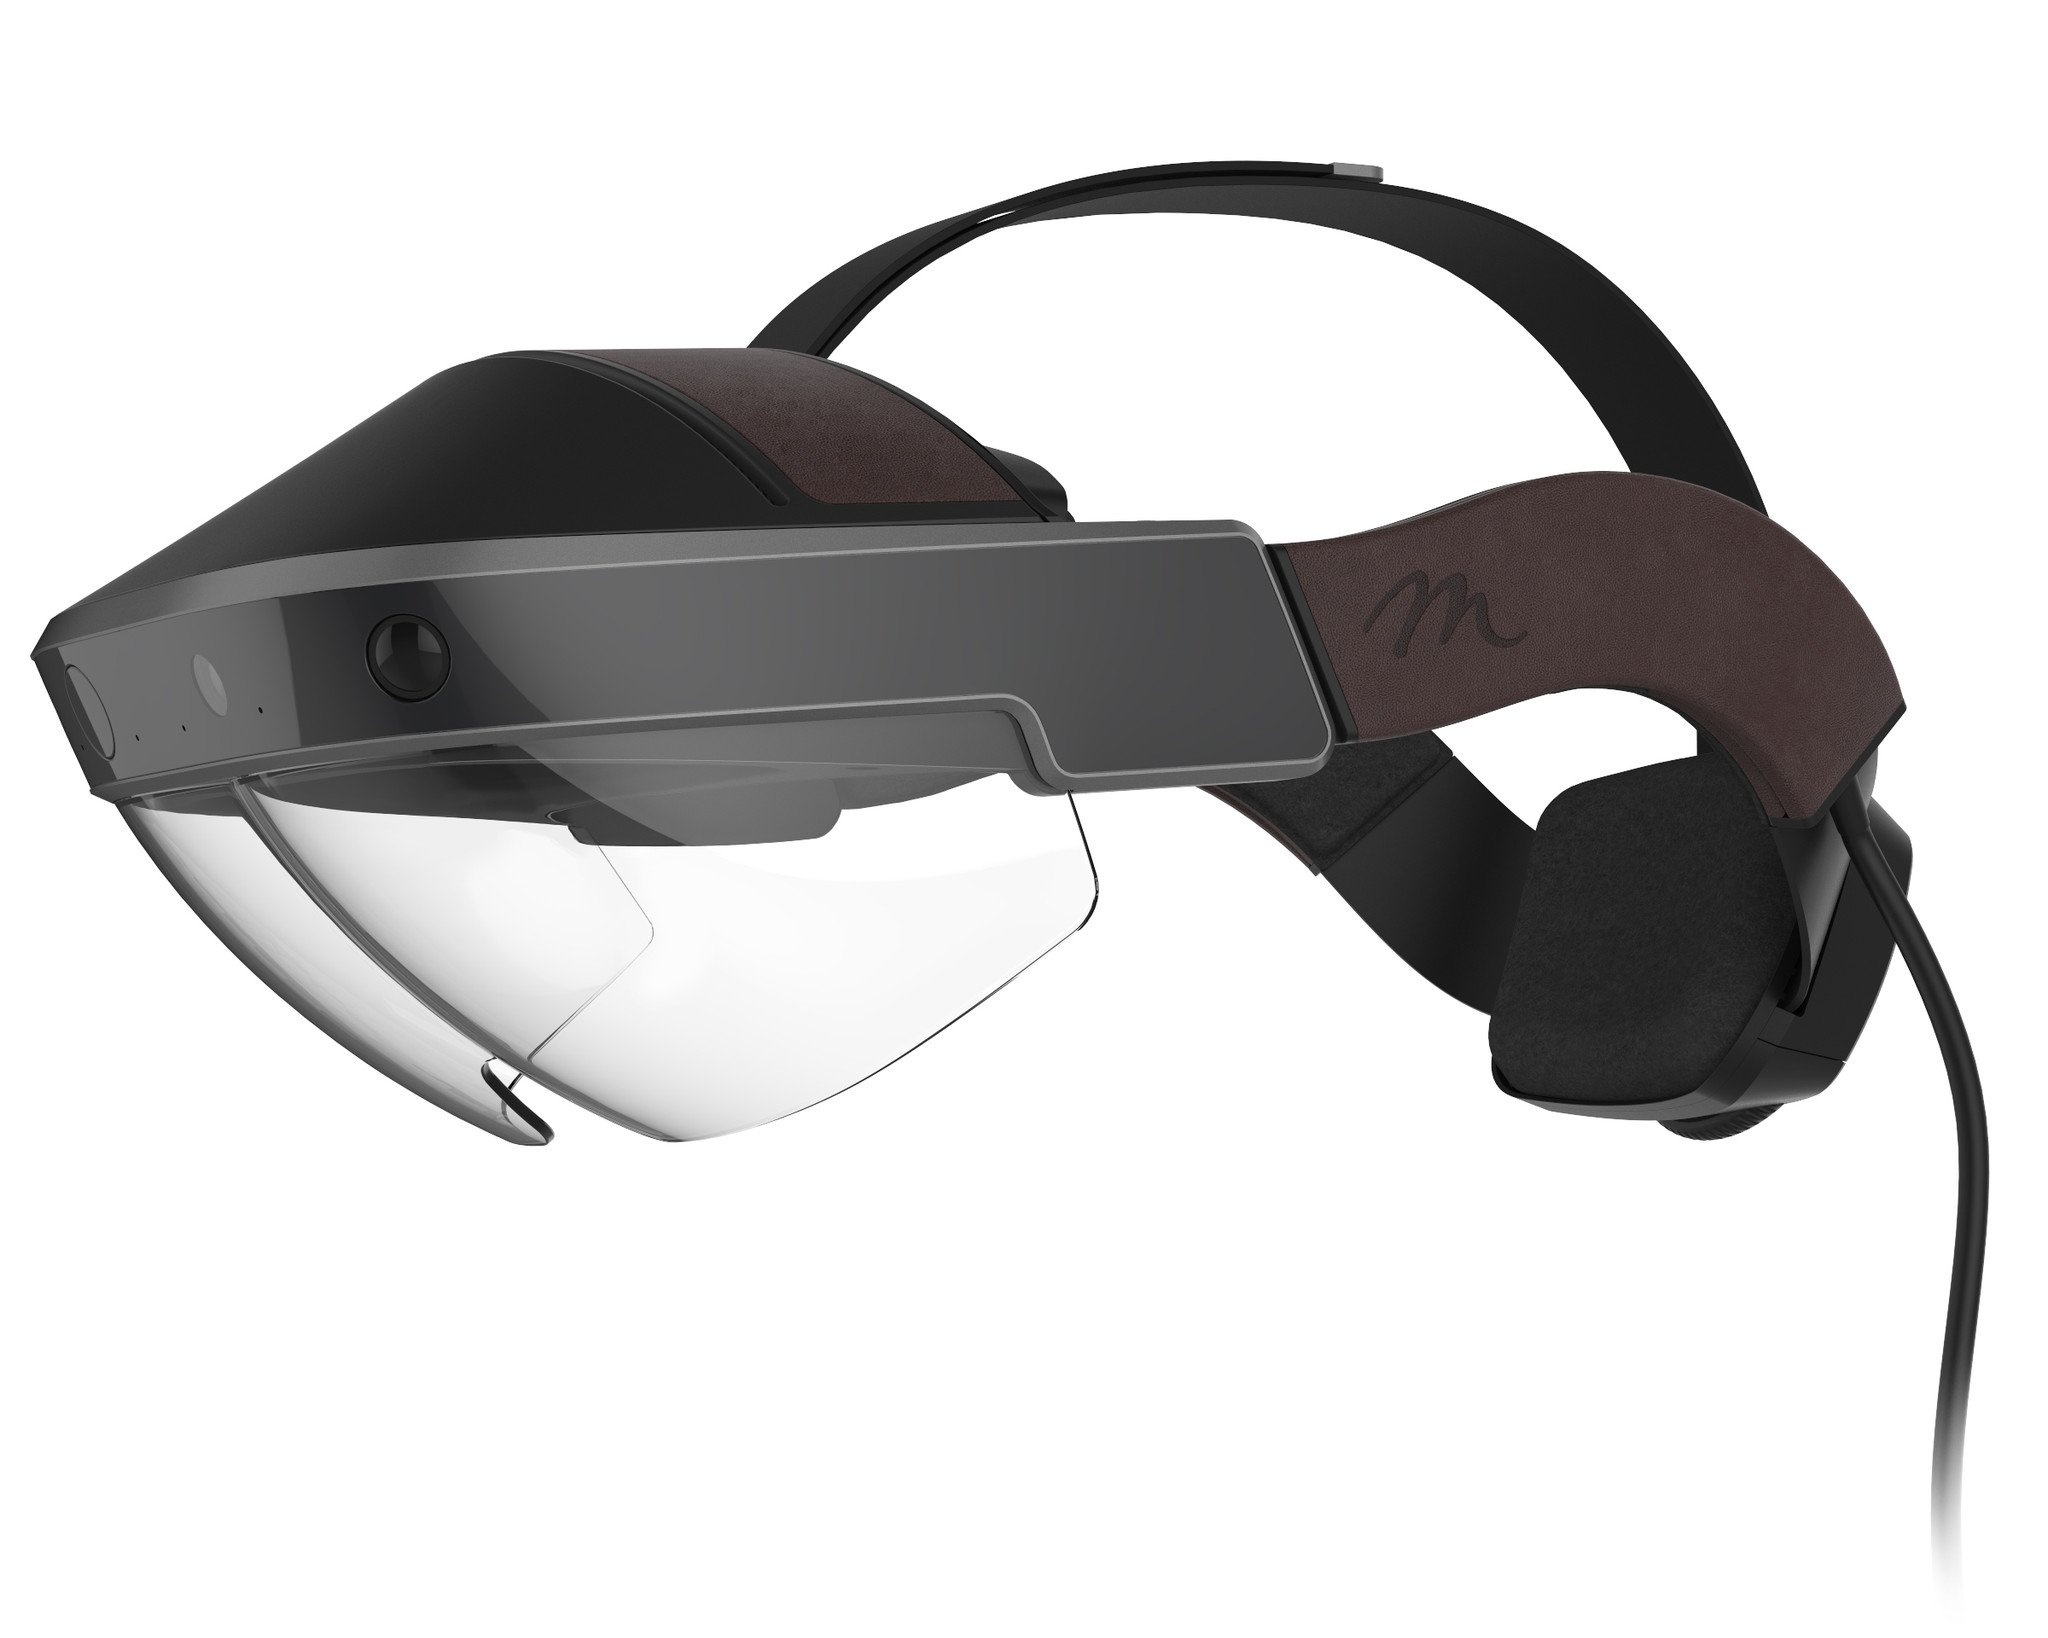
\includegraphics[width=\columnwidth]{images/meta2}
\end{figure}

\newpage


\subsection{Oculus Rift and HTC Vive}\label{subsec:riftvive}
When it comes to holographic devices, the virtual reality headsets have a much larger market share than augmented reality headsets. One major reason for that is the prevalence of VR in the gaming industry. This goes back to the 1990s with the \textit{Virtal Boy} which was developed by Nintendo and continues till today with the \textit{PlayStation VR}.
But VR is not necessarily limited to gaming. There are several of use-cases in medicine, engineering, cinema and entertainment industry. Two of the more popular high-end VR headsets are the \textit{Oculus Rift} (Figure \ref{fig:oculus}) and the \textit{HTC Vive} (Figure \ref{fig:htc}).


\begin{table*}[t]
\normalsize
\caption{Oculus rift vs. HTC Vive}
\centering
\begin{tabular}{p{0.20\linewidth}p{0.40\linewidth}p{0.40\linewidth}}
 & Oculus Rift & HTC Vive\\
 \hline
Display	& OLED & OLED\\
\hline
Resolution & 2160 x 1200 & 2160 x 1200\\
\hline
Refresh Rate & 90Hz & 90Hz\\
\hline
Platform & Oculus Home & SteamVR, VivePort\\
\hline
Field of view & 110 degrees & 110 degrees\\
\hline
Tracking area & 5 x 11 feet & 15 x 15 feet\\
\hline
Built-in audio & Yes & Yes\\
\hline
Built-in mic & Yes & Yes\\
\hline
Controller & Oculus Touch, Xbox One controller & Vive controller, any PC compatible gamepad\\
\hline
Sensors & Accelerometer, gyroscope, magnetometer, Constellation tracking camera. & Accelerometer, gyroscope, Lighthouse laser tracking system, front-facing camera.\\
\hline
Connections & HDMI, USB 2.0, USB 3.0 & HDMI, USB 2.0, USB 3.0\\
\hline
PC Requirements & NVIDIA GeForce GTX 960 / AMD Radeon RX 470 or greater & NVIDIA GeForce GTX 970 /AMD Radeon RX 480 equivalent or greater\\
& Intel Core i3-6100 / AMD FX4350 or greater & Intel Core i5-4590 equivalent or greater\\
& 8GB+ RAM & 4GB+ of RAM\\
& Compatible HDMI 1.3 video output & Compatible HDMI 1.3 video output\\
& 2x USB 3.0 ports & 1x USB 2.0 port\\
& Windows 7 SP1 or greater & Windows 7 SP1 or greater\\

\end{tabular}

\end{table*}

\begin{figure}[ht]
\caption{Oculus Rift}
\label{fig:oculus}
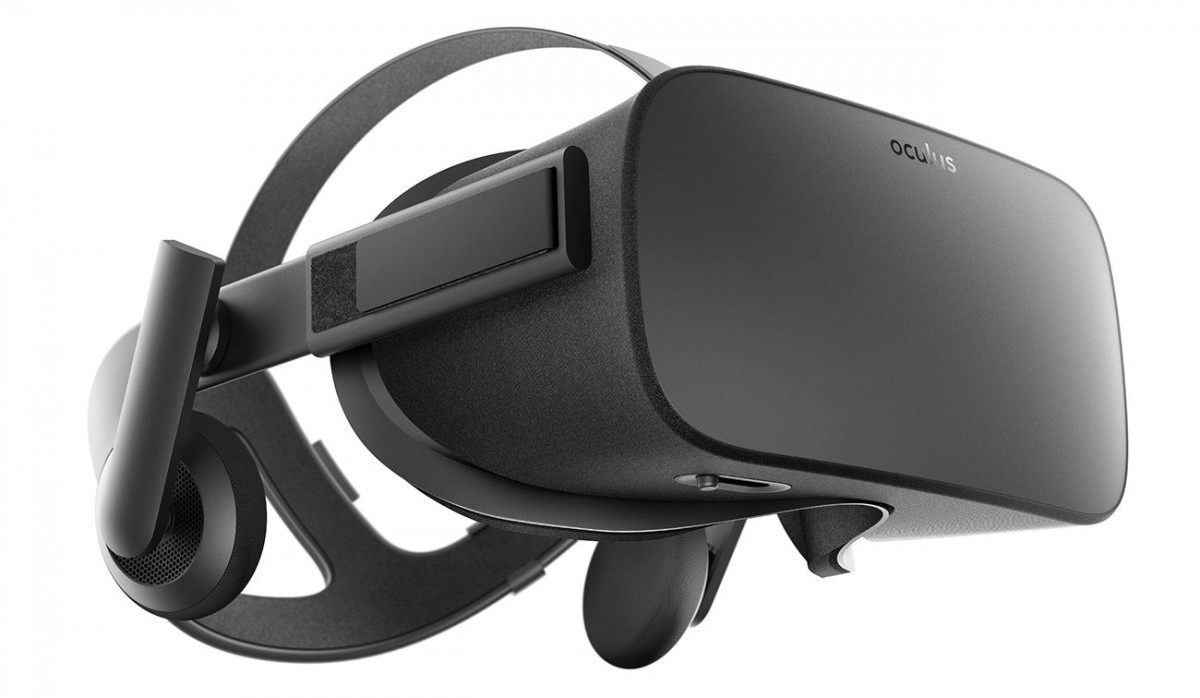
\includegraphics[width=\columnwidth]{images/oculusrift}
\end{figure}


\begin{figure}[ht]
\caption{HTC Vive}
\label{fig:htc}
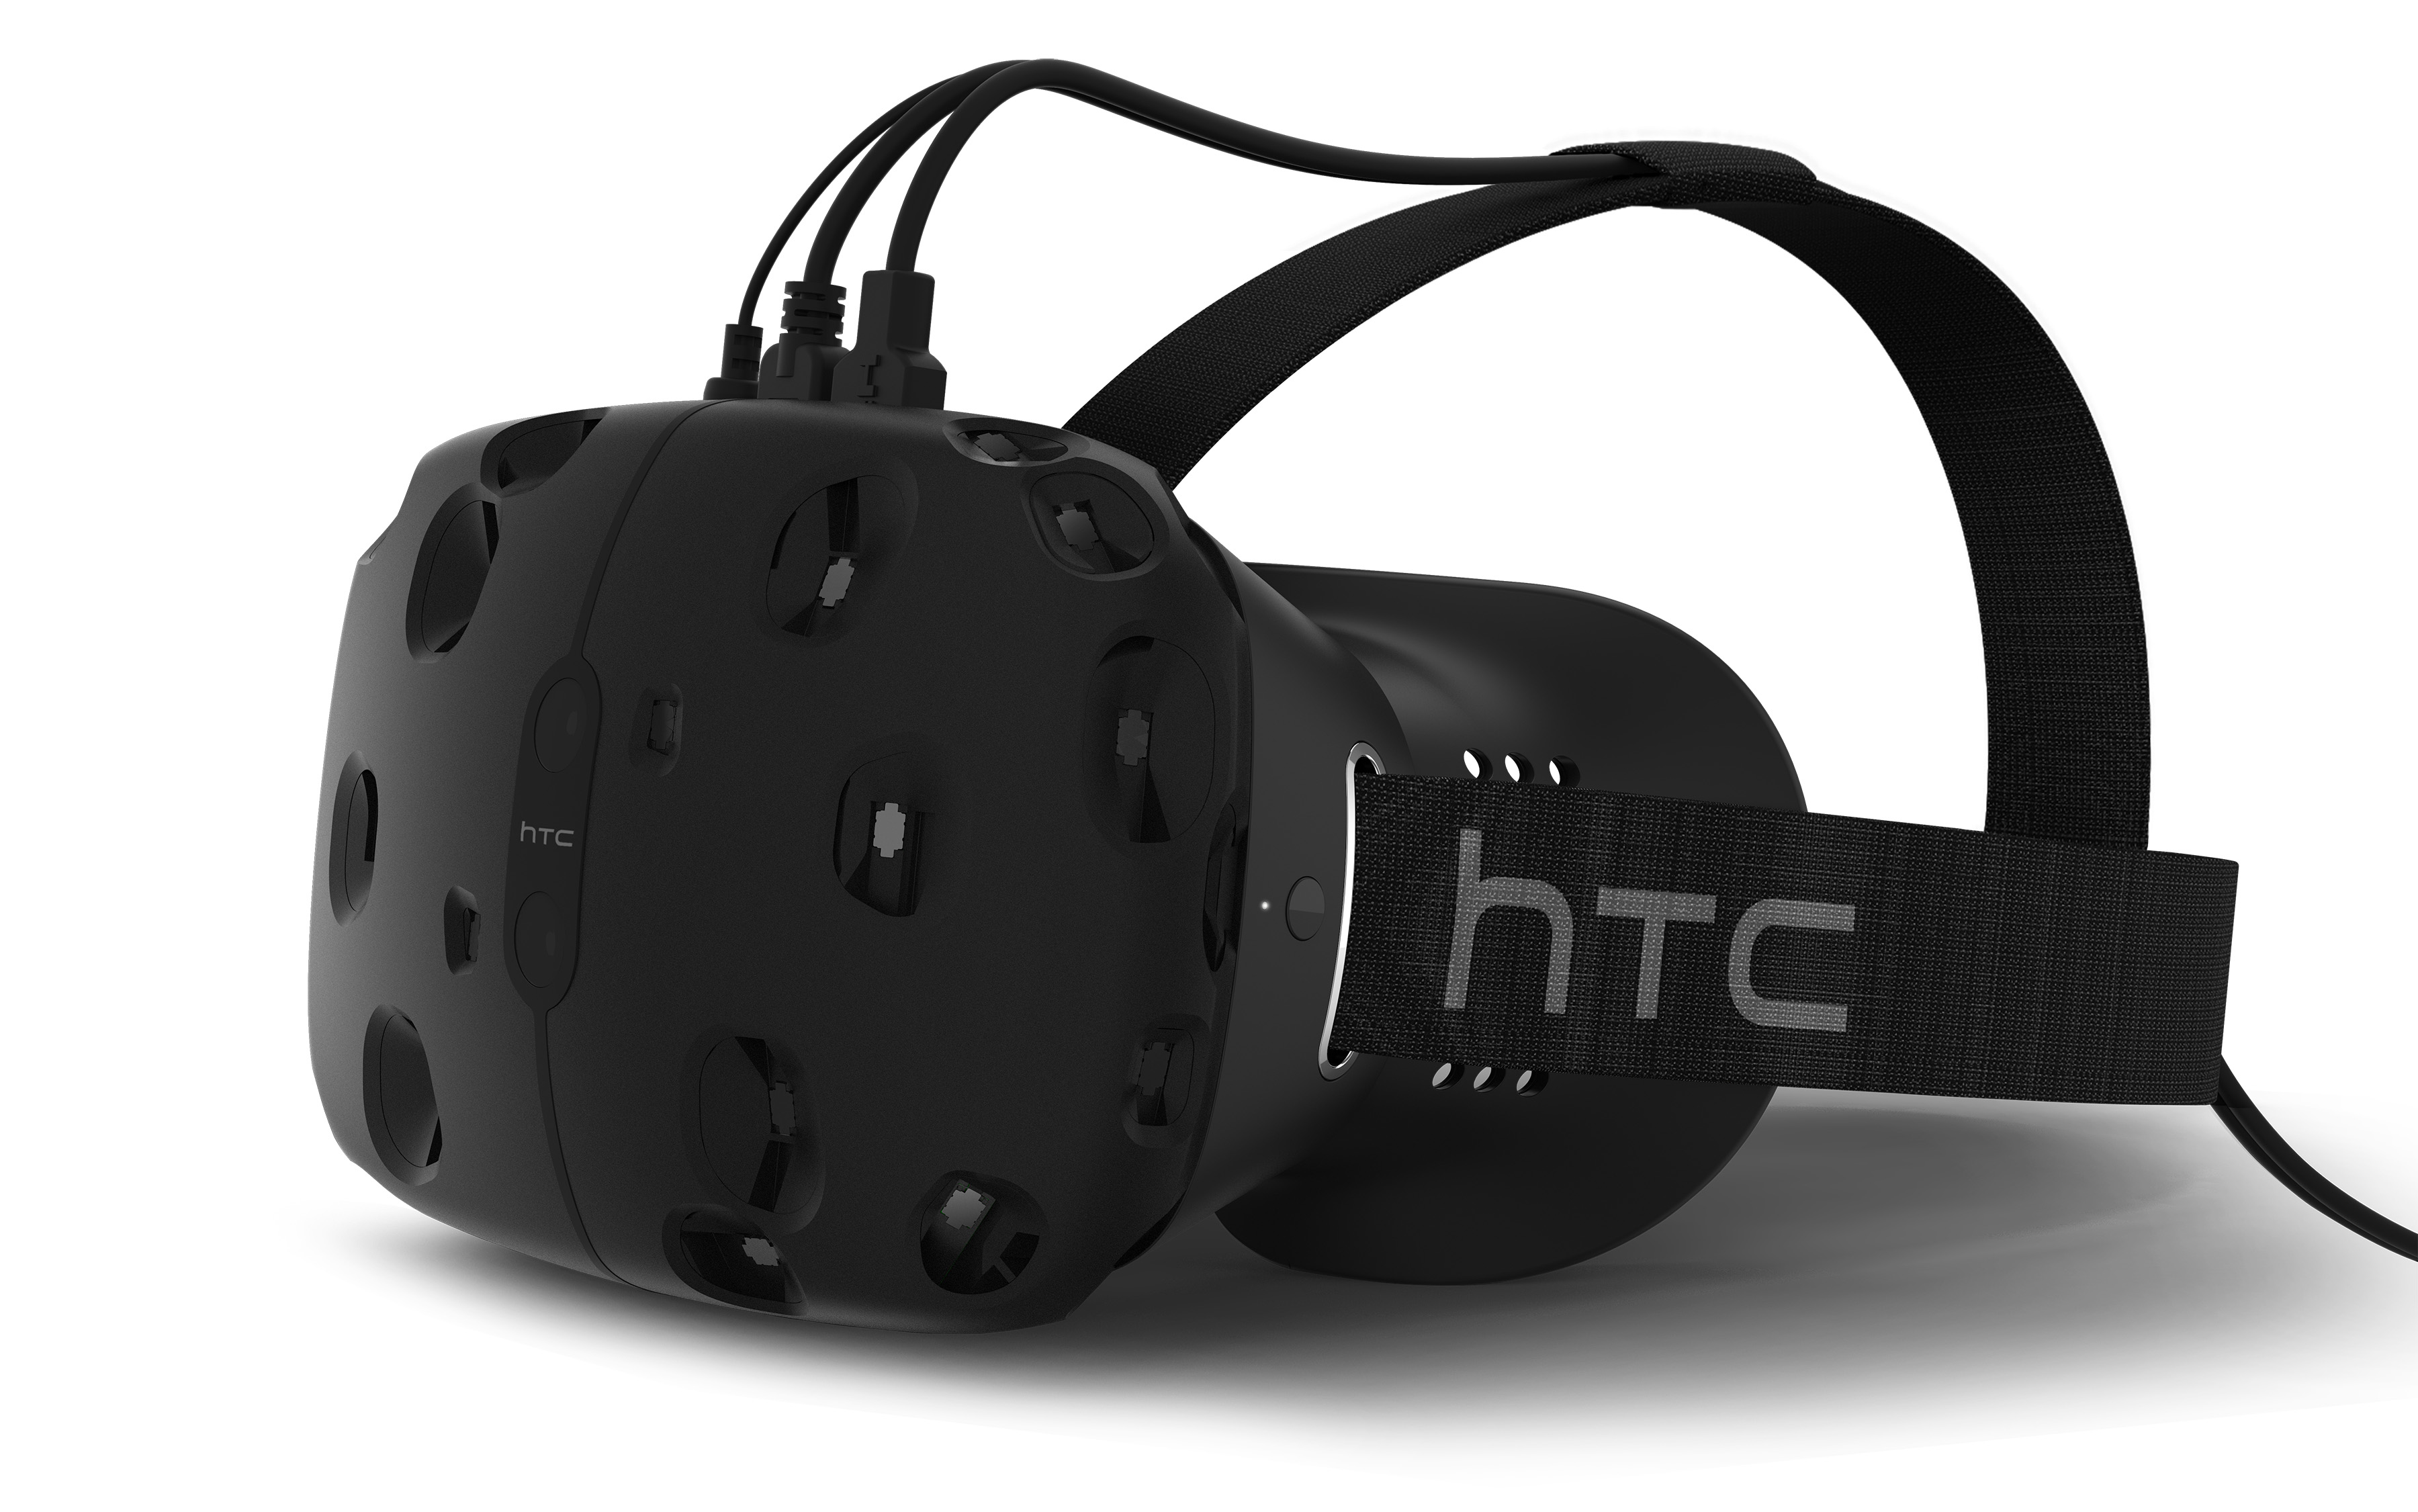
\includegraphics[width=\columnwidth]{images/htcvive}
\end{figure}

\section{Conclusion}\label{sec:end}
In this paper we introduced four different virtual and augmented reality headsets. The virtual reality field is at the moment mostly driven by the gaming industry. The augmented reality field is also capable of becoming an extension for a different kind of gaming experience, but there are a lot of other, perhaps more serious, use-cases that simply cannot be done with VR. There are quite a lot of scenarios where it would be helpful to have some additional information displayed about something in the real world. But for security or other reasons it is often necessary to keep intervisibility. For example in medicine, manufacturing or construction work, the user must have an unhindered view of their work area even if it is only to account for device failure. 
Both of the presented AR devices are capable of superimposing holographic content onto the real world. 

The \textit{Meta 2} (Section \ref{subsec:meta2}) shows holographic objects within arm-reach of the user so that he can interact with them. The \textit{Meta 2} recognizes the hand itself and not separate distinct gestures. 

The \textit{Microsoft HoloLens} (Section \ref{subsec:holoLens}) uses a completely different technology to place holographic objects and interact with them. The holographic objects are attached to real objects and stay there no matter where the user is going. The key feature for this technology is the environment awareness that the \textit{HoloLens} has. So the Range to place holographic is practical unlimited. But to place an holographic object, the \textit{HoloLens} need to have spatial information about this place. That means that the device must scan the environment, than an holographic object can be placed and then the user can walk away from that object and it stays there. To still be able to interact with this object, the \textit{HoloLens} uses a point-and-click interface. One benefit of this method of interacting is, that most people are able to learn it quickly because it is similar to using a mouse on a computer.

When is comes to choosing an augmented reality headset the decision strongly depends on the use-case. For product design or any case where the user has to directly interact with an object, the \textit{Meta 2} would be the right choice. To display holographic information next real objects and keep those information in place, the \textit{Microsoft HoloLens} is the go to device.




%\section{Our Approach}


\end{document}